% !TeX spellcheck = en-US
% !TeX encoding = utf8
% !TeX program = xelatex
% !BIB program = biber

%\documentclass[logoontitle,logoonpages,tabu,supertabular,aspectratio=169]{preney-uwindsor-beamer}
\documentclass[logoontitle,tabu,supertabular,aspectratio=43]{preney-uwindsor-beamer}
%
% NOTE: "Iosevka" and "Charis SIL" fonts are set in main.sty!
%
\usepackage[
bibstyle=numeric-comp,
sorting=nyvt,
natbib=true,
mcite=true,
maxnames=100,
url=true,
isbn=false,
doi=false,
uniquename=init,
giveninits=true,
hyperref=true,
backref=true,
sortcites,
backend=biber
]{biblatex}
\usepackage{url}
\usepackage{hyperref}
\usepackage{main}

\usepackage{booktabs}
\addbibresource{../frostpaper.bib}


\newcommand{\phobos}{\mathit{phobos}}
\newcommand{\deimos}{\mathit{deimos}}
\newcommand{\every}{\mathit{every}}
\newcommand{\spins}{\mathit{spins}}
\newcommand{\spin}{\mathit{spin}}
\newcommand{\moon}{\mathit{moon}}

\newcommand{\meaningof}[1]{\lVert #1 \rVert}
\newcommand{\eventassoc}[1]{ev_{\mathrm{#1}}}
\newcommand{\entityassoc}[1]{e_{#1}}
\newcommand{\wordpred}[1]{\mathit{#1\_pred}}
\newcommand{\wordset}[1]{\mathit{#1\_set}}
\newcommand{\True}{\mathit{True}}
\newcommand{\False}{\mathit{False}}


\newcommand{\discover}{\mathit{discover}}
\newcommand{\discovered}{\mathit{discovered}}
\newcommand{\discoveredby}{\mathit{discovered\ by}}
\newcommand{\discoveredwith}{\mathit{discovered\ with}}
\newcommand{\used}{\mathit{used}}
\newcommand{\hall}{\mathit{hall}}

\newcommand{\relation}[1]{\mathit{#1\_rel}}
\newcommand{\collect}{\mathit{collect}}

\newcommand{\FDBR}[1]{\mathrm{FDBR}({#1})}
\newcommand{\objfdbr}[1]{\mathrm{obj\_fdbr}(\mathit{#1})}
\newcommand{\gatherevs}[1]{\mathrm{gather}({#1})}
\newcommand{\propfdbr}[2]{\mathrm{prop\_fdbr}(\mathit{#1, #2})}
\newcommand{\relationn}[3]{\mathit{#1\_rel_{#2 \rightarrow #3}}}

% Hack to make mintinline work in tabu tables...
% URL: https://tex.stackexchange.com/questions/372053/using-mintinline-inside-tabu/372054
\tabuDisableCommands{%
	\renewcommand\mintinline[2]{\texttt{\detokenize{#2}}}%
}

\providecommand{\emailshane}{peelar@uwindsor.ca}
\title{Scalable, Efficient and Precise Natural Language Processing in the Semantic Web}
\subtitle{Thesis Defence}
\date[December 17 2020]{December 17 2020}
\author[]{\small Shane Peelar \texorpdfstring{\\}{} {\scriptsize\href{mailto:\emailshane}{peelar@uwindsor.ca}}}

%\institute[WEBIST 2020 Conference]{
%	\Large WEBIST 2020 Conference\\ \vspace{1em}
%	\footnotesize Funded by NSERC of Canada
%}

\institute[University of Windsor]{
    %\institute{
    School of Computer Science \texorpdfstring{\\}{}
    University of Windsor \texorpdfstring{\\}{}
    Windsor, Ontario, Canada \texorpdfstring{\\}{}
    %Copyright \copyright{} 2018 \insertshortauthor{}. All Rights Reserved. \texorpdfstring{\\}{}
}


\newcommand{\makesubsectionslide}{
\begin{frame}
	\centering
	\huge
	\insertsubsection
\end{frame}
}

%
% The presentation slide content follows...
%
\begin{document}
	% Set all tabu tables to have 1pt linesep by default...
	\tabulinesep=1pt

	%\partwithoutpage{\inserttitle}
	\section*{Title Page}
	\begin{frame}
	\titlepage
	\end{frame}

  \begin{frame}{Doctoral Committee}
    \begin{itemize}
        \item[] \textbf{External Examiner}: Dr. Diana Zaiu Inkpen %TODO: pronunciation
        \begin{itemize}
            \item[] School of Electrical Engineering and Computer Science
            \item[] University of Ottawa
        \end{itemize}
        \item[] \textbf{External Reader}: Dr. Richard Caron
        \begin{itemize}
            \item[] Department of Mathematics and Statistics
        \end{itemize}
        \item[] \textbf{Internal Reader}: Dr. Jianguo Lu
        \begin{itemize}
            \item[] School of Computer Science
        \end{itemize}
        \item[] \textbf{Internal Reader}: Dr. Pooya Moradian Zadeh
        \begin{itemize}
            \item[] School of Computer Science
        \end{itemize}
        \item[] \textbf{Advisor}: Dr. Richard Frost
        \begin{itemize}
            \item[] School of Computer Science
        \end{itemize}
    \end{itemize}
    \end{frame}

    \begin{frame}[allowframebreaks]{Outline}
       \tableofcontents[hideallsubsections]
    \end{frame}


	\section{Introduction}

    \subsection{Motivation}
    \begin{frame}{\insertsection: \insertsubsection}
        \begin{itemize}
            \item The Internet of Things (IoT) has become an established presence in everyday life
            \begin{itemize}
                \item lightbulbs, televisions, refrigerators, etc \ldots
            \end{itemize}
            \item The Semantic Web offers an opportunity to unify interaction with these devices
            \begin{itemize}
                \item  A platform for storing curated domain-specific information
            \end{itemize}
            \item However, there are a lack of expressive user-friendly ways of interacting with the Semantic Web
            \begin{itemize}
                \item Existing query languages are too low level
            \end{itemize}
            %\item Natural Language is one way of approaching this
%            \item Voice Assistants are now commonplace, especially on smartphones
%            \item It would be ideal if we could query the Semantic Web using speech...
        \end{itemize}
    \end{frame}

    %TODO
    %FROM ICSC 2020
    \subsection{The Semantic Web}
    \begin{frame}{\insertsection: \insertsubsection}
        \begin{itemize}
            \item Commonly referred to as ``Web 3.0''
            \item First coined by Tim Berners-Lee in 2001 \cite{berners2001semantic}
            \item A set of standards by the W3C for interacting with remote {\em triplestores} \cite{w3csemanticweb}
            \begin{itemize}
                \item Triples typically described as {\em subject} - {\em predicate} - {\em object}, all Uniform Resource Identifiers (URIs)
                \item Traditionally entity-based
                \item Example: \texttt{<hall> <discovered> <phobos> .}
            \end{itemize}
            \item Advantages:
            \begin{itemize}
                \item No web scraping required, all machine readable
                \item Simple representation facilitates processing (RDF) \cite{w3c}
                \item Hierarchy of information can be described in OWL \cite{mcguinness2004owl}
            \end{itemize}
            \item Requires {\em reification} for cross referencing
        \end{itemize}
    \end{frame}

    %FROM PROPOSAL
    %TODO: the problem statement should be moved up maybe?
    \subsection{The Problem}
    \begin{frame}{\insertsection: \insertsubsection}

        \begin{block}{Problem Statement}
            There is a strong need for expressive user-friendly modes of interaction to the Semantic Web %  SPARQL is too low-level and not user-friendly.
        \end{block}

        Why is this problem important?
        \begin{itemize}
            \item Accessibility -- people who have disabilities should be able to use the Semantic Web
            %TODO: should be possible for someone to ask their smartphone to start the coffee maker in the kitchen and not have the data ever leave their home.
            \item Ease of Interaction -- users should not need to be experts in software
            \begin{itemize}
                \item Should augment an expert's ability to look for information with provable results
            \end{itemize}
            %TODO: how to express the following?
            %\item Verifiability --
        \end{itemize}

    \end{frame}

    \begin{frame}{\insertsection: \insertsubsection}
    \begin{itemize}
        \item One approach: use a Natural Language Query Interface (NLQI)
        \item Users with certain disabilities particularly stand to benefit from a NL approach
        \begin{itemize}
            \item Modalities: speech, text
        \end{itemize}
        \item Voice Assistants are now commonplace, especially on smartphones
        %TODO: should we discuss the following?
        \begin{itemize}
            \item Find related information (Machine Learning)
            \item Privacy concerns due to centralization
            \item Can't be used in confidential settings
        \end{itemize}
    \end{itemize}
    \end{frame}

    \begin{frame}{\insertsection: \insertsubsection}
        A NLQI approach should:
        \begin{itemize}
            \item Give users control of their data
            \begin{itemize}
                \item Support local knowledge-bases
            \end{itemize}
            \item Work locally using commodity low-power hardware
            \begin{itemize}
                \item NL queries should not need a powerful server for evaluation
            \end{itemize}
            \item Accommodate highly sophisticated queries
            \item Be tolerant of ambiguity
            \item Give the user confidence in the correctness of the result
            %TODO: \item Not be tied to a particular database query language (SPARQL)
        \end{itemize}
    \end{frame}

    %FROM ICSC 2020
    %\subsection{Natural Language is inherently difficult}
    \begin{frame}{\insertsection: \insertsubsection}
        \begin{itemize}
            \item NL is inherently syntactically ambiguous:
            \vspace{0.3em}

            {\hspace{4em} ``\texttt{discovered a moon that spins in 1877}''}
            \begin{itemize}
                \item \texttt{discovered (a (moon that spins)) [in 1877]}
                \item \texttt{discovered (a (moon that (spins [in 1877])))}
            \end{itemize}
            \item Semantic ambiguity also exists: consider the word ``depart''
            \item Users may not enter grammatically correct sentences
            \item Users may misspell words
            \item Users may not clearly state what they mean
            \item The situation does not look good for arbitrary user input!
        \end{itemize}
    \end{frame}

    %FROM ICSC 2020
    \subsection{Constraining the Problem}
    \begin{frame}{\insertsection: \insertsubsection}
        \begin{itemize}
            \item But for NLQIs, the situation isn't as bad as it seems
            \begin{itemize}
            \item The set of possible inputs are constrained to Q\&A-type sentences
            \item A full understanding of the underlying NL is not needed
            \end{itemize}
            %TODO: do we even want to mention this stuff?
            \item NLQIs may be {\em wide} or {\em narrow} in scope
            %TODO: wide: finding related information, narrow: answering the question
            \item Machine Learning is effective for {\em wide}-scoped interfaces
            \item But how can we handle highly specific queries, such as: \texttt{how many moons that orbit a red planet were discovered by nicholson}?
            \item The goal of this research is to produce a framework for NLQIs that can be used with expert systems and highly domain specific databases for precise {\em narrow} queries
        \end{itemize}
    \end{frame}

     %FROM ICSC 2020
    \subsection{Compositional Semantics}
    \begin{frame}{\insertsection: \insertsubsection}
        \begin{itemize}
            \item One approach is to use a NLQI based on a {\em Compositional Semantics} (CS)
            \item The idea: each word in the query has a corresponding mathematical {\em denotation} that allows the query to be treated as a mathematical expression
            \begin{itemize}
                \item \texttt{who discovered a moon} $\Rightarrow$ \texttt{who (discovered (a moon))}
                \item \texttt{hall discovered a vacuumous moon in 1877} \\ $\Rightarrow$ \texttt{hall (discovered (a (vacuumous moon)) [in 1877])}
            \end{itemize}
            \item First described by Richard Montague \cite{Dowty:wall}
            \begin{itemize}
                \item ``\textit{I reject the contention that an important theoretical difference exists between formal and natural languages.}'' (Montague, 1970)
                \item The denotations are formally described in the Typed Lambda Calculus
            \end{itemize}
            %TODO: can use the structure of the query itself to provide insight...
        \end{itemize}
    \end{frame}

    \subsection{Related work}
    \begin{frame}{\insertsection: \insertsubsection}
        Previous attempts at building expressive Natural Language Query Interfaces:
        \begin{itemize}
            \item ORAKEL (2004) \cite{cimiano2007orakel}
            \item QuestIO (2008) \cite{tablan2008natural}
            \item AutoSPARQL (2011) \cite{lehmann2011autosparql}
            \item SQUALL (2014) \cite{ferre2014squall}
            %TODO
            %        \begin{itemize}
            %            \item Interestingly, according to Ferr{\'e}, no systems exist that can handle superlatives %TODO
            %            \item Supports limited prepositions (may pick graph and filter by count: ``in graph'', ``at least 10'')
            %        \end{itemize}
            %TODO: UEV-FLMS
        \end{itemize}
    \end{frame}

%TODO: discuss SPARQL?  perhaps in aux slide...

%TODO: single role assumption?



%TODO: SHORTCOMINGS OF PREVIOUS APPROACHES

    %FROM PROPOSAL
    \subsection{Thesis Statement}
    \begin{frame}{\insertsection: \insertsubsection}
        \begin{block}{Thesis Statement}
            A scalable, efficient, expressive and precise method for processing natural-language queries to the semantic web can be built using a compositional semantics.
        \end{block}

        Need to address:
        \begin{itemize}
            \item Scalability: needs to be able to query very large triplestores
            \item Efficiency: needs to be able to run on low power hardware
            \item Expressiveness: handle superlatives, prepositions, comparatives, negation...
            \item Precision: verification of result
        \end{itemize}

    %TODO: is this not covered by the NL is Inherently Difficult slide?
        Why the thesis is non-obvious:
        \begin{itemize}
            \item Because of criticisms and examples of non-compositionality in language
%            \item However, these criticisms do not apply to NLQIs
%            \item Compositionality is possible for a semantics of queries, which has advantages of modularity and extensibility
        \end{itemize}
    \end{frame}

    %NOTE: 15-25 minutes!!!
    %TODO: sections:
    %Intro (brief)
    % - The problem!!! <-- borrow this from proposal
    % - Why important <-- borrow this from proposal
    % - Why non-trivial <-- borrow this from proposal
    % - Previous work
    % 	- Montagovian/Neo-Davidsonian...
    % 	- FLMS
    %   - UEV-FLMS
    % - Shortcomings of previous work
    % - The new idea
    %Demo (sooner? later?)
    %The five papers
    % - New idea of each paper
    % - How it contributes towards solving the problem
    %Conclusions
    % - We've shown...
    %Future work/next steps
    % - Need an empirical evaluation of the system in a real world setting
    % - QALD/DBPedia

    %SLIDES TO BORROW FROM
    % - MSc: query evaluation?
    % - system architecture?
    % - PhD Comprehensive
    % - PhD Proposal
    % -


    %FROM WEBIST 2020
	\section{Demonstration}
	\begin{frame}{\insertsection}
		A live demonstration of our approach is available at this URL:
		\begin{center}
			\url{http://speechweb2.cs.uwindsor.ca/solarman/demo_sparql.html}
		\end{center}
		Some example queries that can be handled include:
        %TODO: negation examples
		\begin{itemize}
			\item \texttt{what discovered no moon in 1877}
			\item \texttt{what discovered a non moon}
			\item \texttt{allen discovered no moon at no places}
			\item \texttt{what discovered the most moons using no telescopes}
			\item \texttt{phobos and deimos were not discovered by not hall}
			\item \texttt{a person does not exist}
		\end{itemize}
	\end{frame}


   \section{Our Approach}
    \begin{frame}{\insertsection}
        \begin{itemize}
            \item The scoping for the denotations is determined by parsing
            \begin{itemize}
                \item Ambiguous queries will have multiple valid parses
                \item Semantic ambiguity is permitted -- a word may have multiple possible denotations
            \end{itemize}
            \item Let users decide what they mean, rather than try to guess it
            \begin{itemize}
                \item Expose the possible meanings/parses through the interface
            \end{itemize}
            \item Use an {\em event-based} view of information \cite{frost:eswcposter2014}
            \begin{itemize}
                \item Results are {\em auditable} since the result contains the events that justify their inclusion
            \end{itemize}
            \item Constrain the problem to expert systems for domain-specific applications
            \begin{itemize}
                \item Let the {\em wide}-scoped interfaces delegate to {\em narrow} systems where appropriate
            \end{itemize}
            \item Query is an expression in lambda calculus which we then evaluate formally
        \end{itemize}
    \end{frame}

    %TODO: is this background?
    %FROM ICSC 2020
    \subsection{The FDBR}
    \begin{frame}{\insertsection: \insertsubsection}
        \begin{itemize}
            \item The {\em Function Defined by a Binary Relation}
            \item The idea: convert an arbitrary BR into a function by grouping items in the domain together with the sets of elements they map to in the codomain
            \item For example:
            \begin{equation*}
                \relationn{discover}{subject}{object} = \{(\entityassoc{hall}, \entityassoc{phobos}),(\entityassoc{hall},\entityassoc{deimos}),\ldots\}
            \end{equation*}
            \begin{equation*}
                \FDBR{\relationn{discover}{subject}{object}} = \big\{(\entityassoc{hall}, \{\entityassoc{phobos}, \entityassoc{deimos}\}), \ldots\big\}
            \end{equation*}
            \item First used by Frost et. al in 1989 \cite{frost1989constructing} to provide a denotation for binary transitive verbs in MS
        \end{itemize}
    \end{frame}


%TODO: do I really want to try to categorize this stuff?
%	\begin{frame}{\insertsection}
%		\begin{itemize}
%			\item The most popular approaches when dealing with NL involve using Machine Learning (ML)
%			\item Many libraries and frameworks available to facilitate this
%			\item ML is effective at dealing with a wide scope of queries %TODO
%			\item But ML approaches have trouble when things get specific:
%			\begin{itemize}
%				\item \texttt{which person discovered a moon that spins in 1877 with a shiny telescope}
%			\end{itemize}
%			\item Various metrics to evaluate ML approaches: precision, accuracy, recall.. %TODO
%			\item ML approaches try to classify the intent behind a query and present relevant information %TODO, need a citation for that
%		\end{itemize}
%	\end{frame}

    %FROM ICSC 2020
    \section{Original Contributions}

    \begin{frame}{\insertsection}
        In the process of researching the problem, Dr. Frost and I published papers addressing aspects of the thesis statement:
        \begin{itemize}
            \item ``An Extensible Natural-Language Query Interface to an Event-Based Semantic Web Triplestore'' \cite{frost2018extensible}
            \item ``A New Data Structure for Processing Natural Language Database Queries'' \cite{frostpeelar2019}
            \item ``A Compositional Semantics for a Wide-Coverage Natural-Language Query Interface to a Semantic Web Triplestore'' \cite{peelar2020compositional}
            \item ``A New Approach for Processing Natural-Language Queries to Semantic Web Triplestores'' \cite{peelar2020webistjournal}
            \item ``Accommodating Negation in an Efficient Event-Based Natural Language Query Interface to the Semantic Web'' \cite{peelarfrostwebist2020}
        \end{itemize}

    \end{frame}

    \subsection{Superlatives}
    \begin{frame}{\insertsection: \insertsubsection}
        \begin{itemize}
            \item Our approach can accommodate superlative phrases such as ``most'' and ``the most'', including within chained prepositional phrases
            \begin{itemize}
                \item We take ``most'' to mean ``greater than half''
                \item We take ``the most'' to mean ``more than anything else''
            \end{itemize}
            \item For example:
            \begin{itemize}
                \item ``\texttt{who discovered most moons that orbit mars}''
                \item ``\texttt{who discovered the most moons that orbit jupiter}''
            \end{itemize}
            \item Ferré (SQUALL) in 2014 stated no NLQIs can handle this \cite{ferre2014squall}
            %TODO
        \end{itemize}
    \end{frame}

    %TODO: ensure consistent with paper
    \newcommand\biapply{\ensuremath{\mathbin{\ll\mkern-8mu*\mkern-8mu\gg}}}
    \subsection{Query Evaluation}
    \begin{frame}{\insertsection: \insertsubsection}
        %How does $\mathtt{evaluate}$ work?
        How are queries evaluated?
        \begin{itemize}
            \item The event semantics define a filter over the triplestore
            \begin{itemize}
                \item They take in a triplestore as an argument and return answers with respect to those triples
            \end{itemize}
            %\item The notion of event relevance is discussed in my Master's thesis \cite{peelar2016accommodating}
            \item The ``Getts'' semantics:
            \begin{enumerate}
                \item Determine exactly what information is required from the triplestore%, in the form of aggregating the information queried for each ???
                \item Optimize those into as few queries as possible
            \end{enumerate}
            \item These are joined into a 2-tuple, using {\em biapplicative bifunctor} application (operator $\biapply$) to evaluate both semantics in parallel
        \end{itemize}
        \begin{block}{}
            $\mathtt{evaluate}$ takes the queries formed by the Getts semantics and executes them on the triplestore, passing the results into the event semantics in order to obtain an answer.
        \end{block}
    \end{frame}

    %\subsection{System Architecture}
    \begin{frame}{\insertsection: \insertsubsection}
        \begin{figure}[h]
            \centering
            \label{fig1}
            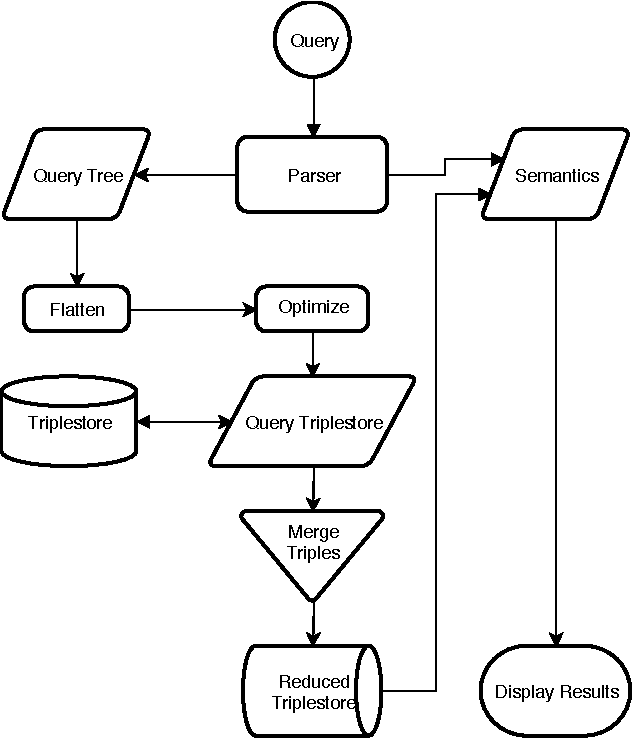
\includegraphics[height=7.3cm]{../images/queryprocess.pdf}
            \caption{System Architecture}
        \end{figure}
    \end{frame}

    %FROM WEBIST 2019 BOOK SERIES:
    %\subsection{Memoization}
    \begin{frame}{\insertsection: \insertsubsection}
        \begin{itemize}
            \item We've shown that it is possible to apply memoization to the query evaluation process itself
            \item The ``Getts'' semantics assigns a unique name to each subexpression of a query
            \item This can be used to re-use results from already evaluated sub-expressions, including in highly ambiguous queries
            \item Can also be used to compute and store FDBRs offline for faster retrieval
            %TODO
        \end{itemize}
    \end{frame}

    \subsection{The $n^2 - n$ Functions Defined by an $n$-ary relation}
    \begin{frame}{\insertsection: \insertsubsection}
    \begin{itemize}
        %TODO
        \item We've shown how to accommodate $n$-ary transitive verbs in a compositional manner
        \begin{itemize}
            \item The new idea: Convert $n$-ary relations to binary relations, then apply the existing FDBR machinery
        \end{itemize}
        \item This makes it possible to query from subject to object, subject to implement, object to year, etc. $n(n - 1) = n^2 - n$ choices.
    \end{itemize}
    \setlength{\tabcolsep}{0.4em} % for the horizontal padding
    \renewcommand{\arraystretch}{1}% for the vertical padding
    \vspace{-1.5em}
    \begin{table}
        \caption{The "Discover'' Relation}
        \centering
        \begin{tabular}{  c c c c c  }
            \hline \hline
            subject & object & date & implement & location \\
            \hline
            \dots & \dots & \dots & \dots & \dots \\
            hall & phobos & 1877 & refractor\_telescope\_1 & us\_naval\_observatory \\
            \dots & \dots & \dots & \dots & \dots \\
            \hline \hline
        \end{tabular}
        \vspace{-1em}
        \label{tab:discover}
    \end{table}
\end{frame}

    \subsection{Applicability to Relational Databases}
    \begin{frame}{\insertsection: \insertsubsection}
    \begin{itemize}
        \item We've shown how our approach can be adapted to relational databases in addition to Semantic Web triplestores
        \item There is a direct correspondence between event-based triplestores and relational databases:
        \begin{itemize}
            \item Event identifier corresponds to the Primary Key
            \item Event type corresponds to the relation or table
            \item Event roles correspond to the columns of the relation
        \end{itemize}
        \item This is owing to the triplestore querying primitives used by the Getts semantics allowing for independence from the triplestore query language itself
        %\item Single Role Assumption
        %TODO
    \end{itemize}
    \end{frame}

    \subsection{Negation}
    \begin{frame}{\insertsection: \insertsubsection}
        \begin{itemize}
            \item We've shown how to accommodate negation with our approach in cases where the Closed World Assumption holds
            \item The new idea: The notion of the complement of an FDBR
            \begin{itemize}
                \item Track the cardinality of FDBRs and the cardinality of the set of all entities during a query
                \item Extend the FDBR operations (union, intersect) to support complements
                \item Requires only the cardinality, not the actual complement, to evaluate many queries
                \item ``drop-in'' denotations for ``not'', ``no'', and ``non''
                \item Denotation for transitive verbs supporting superlatives, prepositional phrases, and negation
            \end{itemize}
            %\item Integrates seamlessly with memoization framework described in \cite{peelar2020webistjournal}
        \end{itemize}
    \end{frame}

%	\section{Our Contribution}
%    \begin{frame}{\insertsection}
%        \begin{itemize}
%            \item The new contribution of this paper is that we can now accommodate negation in the semantics where the CWA holds.
%            \item The new idea: The notion of the complement of an FDBR
%            \begin{itemize}
%                \item Track the cardinality of FDBRs and the cardinality of the set of all entities during a query
%                \item Extend the FDBR operations (union, intersect) to support \texttt{ComplementFDBR}s
%                \item Requires only the cardinality, not the actual complement, to evaluate many queries
%                \item ``drop-in'' denotations for ``not'', ``no'', and ``non''
%                \item Denotation for transitive verbs supporting superlatives, prepositional phrases, and negation
%            \end{itemize}
%            \item Integrates seamlessly with memoization framework described by Peelar in \cite{peelar2020webistjournal}
%        \end{itemize}
%    \end{frame}

%    \begin{frame}{\insertsection}
%    \begin{itemize}
%        \item This makes it possible, where the Closed World Assumption holds, to evaluate Natural Language queries to triplestores having the words ``\texttt{no}'', ``\texttt{not}'', and ``\texttt{non-}''
%        \item Our approach also supports the negation of term-phrases, such as ``\texttt{hall}'', which was missing in previous work
%        \item Double negation: ``\texttt{not not hall discovered not not phobos}''
%        \item ``drop-in'' support: remove the denotations to revert to the OWA
%        \item SQUALL\cite{ferre2013squall}: ``\textit{Which author of Paper42 has not affiliation Salford University?}''
%        \item Our approach: ``\textit{Which author of Paper42 is not affiliated with Salford University?}''
%    \end{itemize}
%    \end{frame}
%	\begin{frame}{\insertsection}
%		\begin{itemize}
%			\item The new contribution of this paper is that we can now handle $N$-ary transitive verbs in a compositional manner
%			\begin{itemize}
%				\item The new idea: Convert $N$-ary relations to binary relations, then apply the existing FDBR machinery
%			\end{itemize}
%			\item This makes it possible to query from subject to object, subject to implement, object to year, etc. $N(N -1) = N^2 - N$ choices.
%			\item We also note that there is a direct correspondence between event-based triplestores and relational databases:
%			\begin{itemize}
%				\item Event identifier corresponds to the Primary Key
%				\item Event type corresponds to the relation or table
%				\item Event roles correspond to the columns of the relation
%			\end{itemize}
%		\end{itemize}
%	\setlength{\tabcolsep}{0.4em} % for the horizontal padding
%	\renewcommand{\arraystretch}{1}% for the vertical padding
%		\vspace{-1.5em}
%		\begin{table}
%			\caption{\footnotesize\normalfont\scshape\\The "Discover'' Relation}
%			\centering
%			\vspace{-0.25cm}
%			\begin{tabular}{  c c c c c  }
%				\hline \hline
%				subject & object & date & implement & location \\
%				\hline
%				\dots & \dots & \dots & \dots & \dots \\
%				hall & phobos & 1877 & refractor\_telescope\_1 & us\_naval\_observatory \\
%				\dots & \dots & \dots & \dots & \dots \\
%				\hline \hline
%			\end{tabular}
%			\vspace{-1em}
%			\label{tab:discover}
%		\end{table}
%	\end{frame}


%	\begin{frame}{\insertsection}
%		\begin{itemize}
%
%			\item This allows us to handle complex linguistic constructs such as chained prepositional phrases
%			%\item This would be far too limiting -- in SPARQL for example, we would not be able to handle chained prepositional phrases
%			\item Instead, gather smaller queries and batch these into larger queries where possible
%			\item The individual denotations are directly derived using set theory, and the answer is as correct as the data
%		\end{itemize}
%	\end{frame}

    \section{Conclusions}
    \begin{frame}{\insertsection}
        \begin{itemize}
            \item We've tackled many features of English that are non-compositional including superlatives, chained prepositional phrases, comparatives, etc... (Expressiveness and Precision)
            \item We've improved our query evaluation computational complexity to polynomial time (Scalability)
            \item Works on low power consumer routers (Efficiency):
            \begin{itemize}
                \item Prototype: \url{https://solarman.inbetweennames.net/}
            \end{itemize}
            \item Works directly within the browser with WebAssembly*
            \begin{itemize}
                \item Prototype: \url{https://speechweb2.cs.uwindsor.ca/solarman-wasm/}
                \item Goal: make the web browser a first class citizen of the Semantic Web
            \end{itemize}

            %\item Imagine browsing the Semantic Web similarly to browsing the WWW
        \end{itemize}
    \end{frame}

	\section{Future Work}
	\begin{frame}{\insertsection}
		\begin{itemize}
            \item Our approach is now ready to be directly benchmarked against other NLQIs
            \begin{itemize}
                \item Question Answering over Linked Data (QALD)
                \item TREC %TODO
                \item YAGO QA benchmark
            \end{itemize}
            \item Non-event based triplestores (Timbr.ai, OWL approaches)
            \begin{itemize}
                \item We have obtained industry interest in our approach
                \item Want to use DBPedia directly as a knowledge store
            \end{itemize}
            \item Evaluation
            \begin{itemize}
                \item Need to conduct a study involving users for evaluation
                \item Ideally benchmarking using established metrics
                \item Want to know what kinds of questions will be people be asking
                \item Aimed for ISWC 2021
            \end{itemize}
		\end{itemize}
	\end{frame}

    %\addtocontents{toc}{\protect\setcounter{tocdepth}{0}}

	\section*{Thank you!}
	\begin{frame}
		\begin{center}
			\huge Thank you for attending!  Questions/comments?
		\end{center}
	\end{frame}

%	\subsection{Overview}
%	\begin{frame}{\insertsection: \insertsubsection}
%	%\begin{block}{Overview}
%	%	Semantics $\leftrightarrow$ Event bridge $\leftrightarrow \{\textit{ML}, \textit{Schemas}\} \leftrightarrow$ Triplestore
%	%\end{block}
%
%	\begin{itemize}
%		\item Must discuss event-based and non-event-based triplestores
%		\item Must discuss reification methods and why they are needed
%		\item Provide motivating examples adding facts to existing info
%	\end{itemize}
%
%
%	\end{frame}

%	\subsection{Previous Work}
%	\begin{frame}{\insertsection: \insertsubsection}
%	Two dominant approaches in NL:
%	\begin{itemize}
%		\item Denotational Semantics: good for \textit{narrow} and \textit{precise} queries (precise answers but requires precise semantics)
%		\item Machine Learning: good for \textit{broad} queries (it finds relevant sections of web pages, but it is only a guess)
%	\end{itemize}
%	Both approaches attempt to translate NL queries into SPARQL\cite{sparql}
%	It is non-trivial because:
%	\begin{itemize}
%		\item Many people are working on the problem
%		\item It is not solved yet
%	\end{itemize}
%	\end{frame}

%	\subsection{Why is it useful? Examples}
%	\begin{frame}{\insertsection: \insertsubsection}
%	\begin{itemize}
%		\item Querying the periodic table (want narrow)
%		\item Querying a wide variety of information (want broad)
%		\item Querying a legal database (want narrow)
%	\end{itemize}
%	\end{frame}

%	\subsection{Hardware acceleration}
%	\begin{frame}{\insertsection: \insertsubsection}
%	I need a section on hardware acceleration, including FPGAs, CUDA, and OpenCL
%	\end{frame}

%	\subsection{Planned publications}
%	\begin{frame}{\insertsection: \insertsubsection}
%	\begin{itemize}
%		\item Spoke in Paris 45 mins seminar
%		\item Spoke during Colloquium Seminars last year for OpenCL
%	\end{itemize}
%	\end{frame}

%	\subsection{FDBR and Goals}
%	\begin{frame}{\insertsection: \insertsubsection}
%	\begin{itemize}
%		\item DBPedia
%		%TODO: must mention SQUALL
%		\item \textbf{No one can do superlatives or compartives} -- quote from 2014 Ferre p.37
%		\item We can do:
%		\begin{itemize}
%			\item Superlative
%			\item Negation
%			\item Preposition
%			\item Comparative
%		\end{itemize}
%		\item FDBR ($n^2 - n$) -- this to be mentioned when going over NLIWoD
%		\item Transitive verbs explicit denotation
%		\item Discuss shortcomings with direct SPARQL translation.
%		%\item Ferre discusses precision in conclusions.
%		%\item Research how SQUALL translates prepositional phrases and the limitations
%	\end{itemize}
%	\end{frame}
%
%	\subsection{ISWC}
%	\begin{frame}{\insertsection: \insertsubsection}
%	\begin{itemize}
%		%\item NLIWoD is a specific workshop, was absorbed into ISWC
%		\item The paper deals with the main shortcomings of MS
%		\item Reawakening interest in MS
%		%\item Why did MS fall out of favour? go over this?  was it mentioned in Squall 2014?
%		%\item Richard will send citation for Ferre Squall 2014
%	\end{itemize}
%	\end{frame}



	%\part{Introduction}
	%==========================================================================

	%\part{References}
	%\sectionwithouttoc{Questions}
	%\begin{frame}{\insertsection}
	%  Questions\par
	%\end{frame}

    \section*{References}
	\begin{frame}[allowframebreaks]{References}
	\printbibliography
	\end{frame}

    %\appendix
    \section*{Appendix}
	%\section*{Appendix}
    \subsection{Example query}
    \begin{frame}{\insertsection: \insertsubsection}
        \begin{itemize}
            %TODO: want a slide showing 3 moons discovered with 2 telescopes
            % and nicholson's discoveries
            % want to walk through how they work

            \item Example: the moons that were discovered by Nicholson
            \item moons: \texttt{lysithea, ananke, carme, sinope}
            \item implements: \texttt{hooker\_telescope, refractor\_telescope\_2}
            \item \texttt{ananke, carme, lysithea-hooker\_telescope}
            \item \texttt{sinope-refractor\_telescope\_2} (also used to discover \texttt{almathea})
        \end{itemize}
    \end{frame}

    \subsection{Contributions to the SpeechWeb project}
    \begin{frame}{\insertsection: \insertsubsection}
    \begin{itemize}
		\item Joined the SpeechWeb project in 2014
        \begin{itemize}
            \item Other students also working on it at that time: the parser, ``Gangster'' semantics
            \item Wrote the demonstration program used by Frost at ESWC
        \end{itemize}
        \item Showed that chained prepositional phrases can be handled in a CS (Masters Thesis) \cite{peelar2016accommodating}
        \item Showed how the word ``by'' can be treated like a preposition
        \item Showed how to accommodate $n$-ary transitive verbs in an event semantics
        \item Showed how the FDBR can be used to answer other ``non-compositional'' queries (superlatives, comparatives)
    \end{itemize}
    \end{frame}

    \begin{frame}{\insertsection: \insertsubsection}
    \begin{itemize}
        \item Showed it is possible to memoize the semantics to improve the asymptotic complexity of evaluation significantly \cite{peelar2020webistjournal}
        \item Showed that it is possible to accommodate negation efficiently
        \item Improved X-SAIGA parser so that it can be used in the browser
        \item Showed that the approach works on low power hardware (consumer routers)
        \item Voice-enabled interface supporting speech input and output
        \item Tackled every non-compositional feature that has been raised by others
    \end{itemize}
    \end{frame}

    %FROM ICSC 2020
    \subsection{Master's thesis contributions}
    \begin{frame}{\insertsection: \insertsubsection}
        \begin{itemize}
            \item It was realized by Peelar and Frost that the FDBR could be used to answer many kinds of queries in NL
            \item In 2016, Peelar showed that it is possible to unify the treatment of complex English constructs (UEV-FLMS) using the FDBR \cite{peelar2016accommodating}
            \begin{itemize}
                \item A query can be thought of as a filter over the underlying database
            \end{itemize}
            \item In particular, it could be used to accommodate chained Prepositional Phrases, which was a common critique of MS approaches
        \end{itemize}
    \end{frame}

        %FROM ICSC 2020
    \subsection{Event-based triplestores}
    \begin{frame}{\insertsection: \insertsubsection}
        \begin{itemize}
            \item The {\em subject} of a triple is the URI of an \textit{event} in which something took place
            \item Data is already {\em reified}, extra information directly accessible
            \item Can add new columns and rows to a relation easily
        \end{itemize}

        Example (N-Triples format \cite{w3cntriples}, full URI omitted):
        \begin{block}{}
            \hspace{5em}\texttt{<event1045> <subject>\phantom{qqq}<hall> .}

            \hspace{5em}\texttt{<event1045> <object>\phantom{qqqq}<phobos> .}

            \hspace{5em}\texttt{<event1045> <type>\phantom{qqqqqq}<discover\_ev> .}

            \hspace{5em}\texttt{<event1045> <year>\phantom{qqqqqq}<1877> .}

            \hspace{5em}\texttt{<event1045> <location>\phantom{qq}<us\_naval\_observatory> .}

            \hspace{5em}\texttt{<event1045> <implement>\phantom{q}<refractor\_telescope\_1> .}
        \end{block}

    \end{frame}

    \subsection{Querying the Semantic Web}
    \begin{frame}{\insertsection: \insertsubsection}
        \begin{itemize}
            \item Many ways to query Semantic Web triplestores
            \begin{itemize}
                \item SPARQL, Triple Pattern Fragments (Linked Data), SQL, etc \ldots
            \end{itemize}
            \item However, these query languages are not suitable for user-interfaces
            \item Example SPARQL query:
        \end{itemize}
        \begin{block}

            \ttfamily

            PREFIX sol: <http://solarman.richard.myweb.cs.uwindsor.ca\#>

            SELECT ?ev ?ent WHERE \{

            \hspace{5em}    ?ev sol:type sol:membership .

            \hspace{5em}    ?ev sol:subject ?ent .

            \hspace{5em}    ?ev sol:object sol:moon .

            \}
        \end{block}
    \end{frame}

    \subsection{Advantages of Compositional Semantics}
    \begin{frame}{\insertsection: \insertsubsection}
        CS has a few advantages when dealing with structured queries:
        \begin{itemize}
            \item Extensible: new denotations able to be added without modifying existing ones
            \item Syntactic categories can be type checked: ``\texttt{hall}'' and ``\texttt{a person}'' have the same type and can be substituted
            \item Expressive: small set of rules define an infinite language
            \item Can be used directly with an Executable Attribute Grammar \cite{frost1989constructing} to ``execute'' NL as if it were a programming language
            %TODO: want a slide for this!
            \item Derivations directly in the language itself
            \item The result of the query is as correct as the underlying database
        \end{itemize}
    \end{frame}

    \subsection{Why CS isn't used more}
	\begin{frame}{\insertsection: \insertsubsection}
		\begin{itemize}
			\item So, why aren't CS used more?  Several reasons:
			\begin{itemize}
				\item Complex linguistic constructs have been traditionally hard to handle
				\item The CS as described by Montague is computationally intractable
				\item Montague's denotation for transitive verbs is very complicated
				\item Not robust with respect to user input
				\item Need to translate the NL query to some kind of structured query language \cite{hoffart2013yago2}
				\begin{itemize}
					\item Underlying query language needs to be complex enough to support NL
				\end{itemize}
			\end{itemize}
		\end{itemize}
	\end{frame}

	\begin{frame}{\insertsection: \insertsubsection}
		\begin{itemize}
			\item There have been major advancements to address these shortcomings:
			\begin{itemize}
			\item In 1989, Frost et. al described FLMS, a tractable version of Montague's semantics, along with a denotation for $2$-ary transitive verbs \cite{frost1989constructing}
			\item In 2014, it was shown that direct translation to an underlying query language is not required (EV-FLMS) \cite{frost2014denotational}
			\item In 2016, Peelar showed that chained prepositional phrases can be handled in a CS (Masters Thesis) \cite{peelar2016accommodating}
			%\item In YEAR, Frost and Peelar showed that superlatives can also be handled %TODO
			\item In 2020, we showed that $N$-ary transitive verbs can be handled compositionally \cite{peelar2020compositional}
            \item In 2020, we showed it is possible to memoize the semantics to improve the asymptotic complexity significantly \cite{peelar2020webistjournal}
            \item In 2020, we now show it is possible to accommodate negation efficiently as well
			\end{itemize}
		\end{itemize}
	\end{frame}

    \subsection{Query Evaluation}
	\begin{frame}{\insertsection: \insertsubsection}
		\begin{itemize}
			\item We have shown that it is not necessary to directly translate the query to an underlying query language \cite{frost2014demonstration}
			\begin{itemize}
				\item The denotation itself contains a small set of queries for the information they need
				\item Batch these smaller queries together
			\end{itemize}
			\item Three simple ``query'' functions used, can be implemented in any query language
			\begin{itemize}
				\item Implementable directly in SPARQL, Triple Pattern Fragments (LDF), and even SQL
			\end{itemize}
		\end{itemize}
	\end{frame}

    \subsection{Implementation}
	\begin{frame}{\insertsection: \insertsubsection}
		\begin{itemize}
			\item Our implementation is written entirely in Haskell
			\item It is able to be used even on low power devices, such as consumer routers
			\begin{itemize}
				\item \url{https://solarman.inbetweennames.net}
			\end{itemize}
			\item The FDBRs are able to be generated offline or on the fly
			\item The semantics are completely memoized for efficient computation
			\item The code is completely open source, available on Hackage \cite{xsaiga}
            \item Now can run entirely within the web browser:
            \begin{itemize}
                \item \url{https://speechweb2.cs.uwindsor.ca/solarman-wasm/}
            \end{itemize}
		\end{itemize}
	\end{frame}

    \subsection{Lambda Calculus}
    \begin{frame}{\insertsection: \insertsubsection}
    \begin{itemize}
        \item Universal model of computation
        \item Consider the function: $\mathrm{add} = (\lambda x.(\lambda y.x + y))$
        \item Example application:
    \end{itemize}
    \begin{equation*}
        \begin{split}
            \ \mathrm{add}\ 3\ 4 =&\ (\lambda x.(\lambda y.x + y))\ 3\ 4 \\
            =\!\Rightarrow &\ (\lambda y.3 + y)\ 4 \qquad\mathrm{This\ is\ an\ example\ of\ beta\ reduction}\\
            =\!\Rightarrow &\ 3 + 4
        \end{split}
    \end{equation*}

    \begin{equation*}
        \begin{split}
            &\mathrm{add\_three} = \mathrm{add}\ 3 = \lambda y. 3 + y \qquad\mathrm{Partial\ application\ of\ add\ returns\ a\ function}\\
            &\mathrm{add\_three}\ 6 =\!\Rightarrow \mathrm{add}\ 3\ 6 =\!\Rightarrow 9
        \end{split}
    \end{equation*}
    \end{frame}

    \subsection{Montague Semantics}
    \begin{frame}{\insertsection: \insertsubsection}
        \begin{itemize}
            \item Montague was the first person to propose that two phrases of the same class were of the same type
            \item Also first to propose that a proper noun denotes a function, not an entity
            \item Described semantics in the Typed Lambda Calculus
            \item Common Nouns are denoted by sets of entities
            \item Term-phrases take a set of entities and return a boolean value
            \begin{itemize}
                \item Proper Nouns
                \item Determiner Phrases (e.g, ``\texttt{a moon}'')
            \end{itemize}
        \end{itemize}
    \end{frame}

    %\subsection*{Montague Semantics}
    \begin{frame}{\insertsection: \insertsubsection}
        \centering
        Note: $\meaningof{w}$ is the denotation of $w$

        \begin{equation*}
            \begin{split}
                &\meaningof{\spin} = \wordpred{\spins} \\
                &\meaningof{\phobos} = \lambda p. p\ e_\mathrm{phobos} \\
            \end{split}
        \end{equation*}
        \begin{equation*}
            \begin{split}
                & \meaningof{\phobos \ \spins} \\
                =\!\Rightarrow&  \meaningof{\phobos}\ \meaningof{\spins} \\
                =\!\Rightarrow&  \lambda p. p \ \entityassoc{phobos} \ \meaningof{\spins} \\
                =\!\Rightarrow&  \lambda p. p \ \entityassoc{phobos} \ \wordpred{\spins}\\
                =\!\Rightarrow&  \wordpred{\spins} \ \entityassoc{phobos} \\
                =\!\Rightarrow&  \True
            \end{split}
        \end{equation*}

    \end{frame}

    \begin{frame}{\insertsection: \insertsubsection\ (con't)}

        \begin{equation*}
            \meaningof{\every} = \lambda p.\lambda q. \  \forall x \  (p \  x \Rightarrow q \  x) \\
        \end{equation*}

        \begin{equation*}
            \begin{split}
                & \meaningof{\every \  \moon \  \spins} \\
                =\!\Rightarrow&  (\meaningof{\every} \  \meaningof{\moon}) \  \meaningof{\spins} \qquad(\mathrm{from}\ \mathrm{syntactic}\ \mathrm{parsing}) \\
                =\!\Rightarrow&  (\lambda p.\lambda q.\ \forall x (p \  x \Rightarrow q \  x) \  \wordpred{\moon}) \  \wordpred{\spins} \\
                =\!\Rightarrow&  (\lambda q.\ \forall x \  (\wordpred{\moon} \   x \Rightarrow q \   x)) \  \wordpred{spins} \\
                =\!\Rightarrow&  \forall x \  \wordpred{\moon} \   x \Rightarrow \wordpred{spins} \   x \\
                =\!\Rightarrow&  \True \qquad(\mathrm{every}\ \mathrm{moon}\ \mathrm{in}\ \mathrm{the}\ \mathrm{universe \ of\ discourse}\ \mathrm{spins}\ (\mathit{costly!}))
            \end{split}
        \end{equation*}
        \centering

        Note: $\meaningof{\phobos}$ has same type as $\meaningof{\every\ \moon}$

    \end{frame}

    \subsection{Montague’s treatment of transitive verbs}
    \begin{frame}{\insertsection: \insertsubsection}
        Transitive verbs are left uninterpreted until the rest of the phrase has been interpreted and reduced as far as possible.

        The expression is then rewritten to another lambda expression using a syntactic
        sigma σ rule. See page 216 of \textit{Dowty, Wall and Peters 1981}\cite{Dowty:wall} .

        \begin{itemize}
            \item Complicated and difficult to implement

            \item No explicit denotation for transitive verbs

            \item Therefore no denotation, for example, for ``discovered phobos''
        \end{itemize}
    \end{frame}


    \subsection{SQUALL}
    \begin{frame}{\insertsection: \insertsubsection}
        \begin{itemize}
            \item A Constrained Natural Language (CNL) for the Semantic Web
            \item Translates NL queries directly to SPARQL using a CS
            \item Limited support for prepositions, superlatives
            \item Coverage of English is limited to non-chained constructs
            \item ``Which author has affiliation...'', ``Which author is affiliated with...''
        \end{itemize}
    \end{frame}

    \subsection{Blackburn and Bos approach to Transitive Verbs}
    %\subsection*{Blackburn and Bos approach to Transitive Verbs}
    \begin{frame}{\insertsection: \insertsubsection}
        \begin{equation*}
            \meaningof{discover} = \lambda z. z(\lambda xy. \wordpred{\discover}(y, x))
        \end{equation*}

        \centering
        Works for 2-place transitive verbs (see \textit{Frost ACM Surveys}\cite{frost2006realization})
    \end{frame}

    \begin{frame}{\insertsection: \insertsubsection\ (con't)}
        \centering

        MS: Direct Evaluation of NL Queries w.r.t. Datastore

        {
            \color{orange}
            ``Who (stole (a car) [in (1918 or 1920), in (a (borough (of New\_York)))])?''
        }

        $\Downarrow\quad\Downarrow\quad\Downarrow\quad\Downarrow\quad\Downarrow\quad\Downarrow\quad\Downarrow\quad\Downarrow\quad\Downarrow\quad\Downarrow\quad\Downarrow$

        {\small$\lambda\ldots ( \lambda\ldots ( \lambda\ldots \lambda\ldots) [\lambda\ldots (\lambda\ldots \lambda\ldots \lambda\ldots), \lambda \ldots(\lambda\ldots(\lambda\ldots ( \lambda\ldots \lambda\ldots)))])$}

        $\Uparrow\quad\Uparrow\quad\Uparrow\quad\Uparrow$

        \textbf{TRIPLESTORE}

        Where $\lambda\ldots$ are functions (which are the denotations of English words)

        {
            \color{red}
            Some functions are defined
        }
        $\Uparrow$
        {
            \color{red}
            in terms of triplestore retrieval operations
        }
    \end{frame}

    \subsection{Flow of NL query process}
    \begin{frame}{\insertsection: \insertsubsection}
        \small
        \centering
        ``who used a telescope in 1877''
        \[\Downarrow \qquad \Downarrow \qquad \Downarrow \]
        \[ \mathtt{evaluate} ( \mathtt{who} \biapply (\mathtt{used''} \biapply \left(\mathtt{a} \biapply \mathtt{telescope}\right) \biapply \]
        \[ \mathtt{gatherPreps} \left[ \mathtt{in'} \biapply \mathtt{make\_year}\ \mathtt{1877}\right] ))  \]
        \[\Downarrow \qquad \Downarrow \qquad \Downarrow \]
        %mention that a NL query is fundamentally a filter over a dataset
        %\[\mathtt{evaluate} \left(\mathtt{who}\ \left(\mathtt{used''}\ \left(\mathtt{a}\ \mathtt{telescope}\right)\ \left[ \mathtt{in'}\ \mathtt{1877}\right] \right),getts...\right) \]
        \[\mathtt{evaluate}\ \mathtt{triplestore} \left(\mathtt{filter},\mathtt{getts}\right) \]
        %expand on biapplicative bifunctor
        \[\Downarrow \qquad \Downarrow \qquad \Downarrow \]
        \[\mathtt{retrieve}\ \mathtt{getts} \longleftrightarrow \mathtt{triplestore} \]
        %should an FDBR be a set? check the literature.  NO: evaluate is not math, it is algorithm.

        %\texttt{...(event1045, subject, hall), (event1045, year, 1877), (event1045, type, discover\_ev)...}
    \end{frame}

    %TODO: neo-davidsonian, davidsonian, Montague's approach

    \begin{frame}{\insertsubsection\ (con't)}
        \centering
        \[\mathtt{retrieve}\ \mathtt{getts} \longleftrightarrow \mathtt{triplestore} \]
        \[\Downarrow \qquad \Downarrow \qquad \Downarrow \]
        %\[\left[\ldots\left(hall, \left[event1045\right]\right)\ldots\right]\]
        \texttt{...(event1045, subject, hall), (event1045, year, 1877), (event1045, type, discover\_ev)...}
        \[\Downarrow \qquad \Downarrow \qquad \Downarrow \]
        \[\mathtt{filter} \longrightarrow \left[\ldots\left(hall, \left[event1045\right]\right)\ldots\right]\ \mathrm{(FDBR)}\]
        \[\Downarrow \qquad \Downarrow \qquad \Downarrow \]
        hall
    \end{frame}

    %FROM WEBIST 2020
    \subsection{Negation}
    \begin{frame}{\insertsection: \insertsubsection}
        \begin{itemize}
            \item RDF is based on the Open World Assumption, which can be summarized as: \linebreak
            ``\textit{The absence of evidence cannot be construed as being evidence of absence.}''
            \item This makes negation tricky to work with:
            \begin{itemize}
                \item Obtaining the cardinality of a set may not be possible
                \item Or it may be so large that it is not practical to work with
            \end{itemize}
            \item But the Closed World Assumption may still hold for domain specific applications
            \item \textbf{How can we support use cases where the CWA holds?}
        \end{itemize}
    \end{frame}

    \subsection{Bi-functors}
    \begin{frame}{\insertsection: \insertsubsection}
        \begin{itemize}
            \item In Category Theory, a Functor is a map between categories
            \item A bi-functor is a functor from a product category to another category (like a cartesian product e.g, $\mathbb{Q} \times \mathbb{Q} \rightarrow \mathbb{R}$)
            \item In Functional Programming, a Functor is something that can be ``mapped'' over
            \begin{itemize}
                \item \texttt{fmap :: (Functor p) => (a -> b) -> p a -> p b}
                \item e.g, the elements of a list, or the nodes of a tree, or a stream of input
            \end{itemize}
            \item A Bi-Functor takes on a similar meaning:
            \begin{itemize}
                \item \texttt{bimap :: (Bifunctor p) => (a -> b) -> (c -> d) -> p a c -> p b d}
                \item e.g, to map over a pair of values \texttt{(a,b)}, where \texttt{p = (,)}
            \end{itemize}
        \end{itemize}
    \end{frame}

    \subsection{Applicative Functors}
    \begin{frame}{\insertsection: \insertsubsection}
            In Functional Programming, an Applicative Functor wraps function application
            \begin{itemize}
                \item \texttt{(<*>) :: Applicative p => p (a -> b) -> p a -> p b}
                \item \texttt{pure :: Applicative p => a -> p a}
            \end{itemize}
            E.g., useful for error handling:
            \texttt{maybe\_function <*> maybe\_value} could evaluate to either another value or a special error value \texttt{Nothing}
            \begin{itemize}
                \item Note that it must satisfy the Applicative Laws
            \end{itemize}
    \end{frame}

    \subsection{Bi-Applicative Bi-Functors}
    \begin{frame}{\insertsection: \insertsubsection}
            A Bi-applicative Bi-functor is the same concept applied to a Bi-Functor:
            \begin{itemize}
            \item \texttt{(<<*>>) :: Biapplicative p => p (a -> b) (c -> d) -> p a c -> p b d}
            \item \texttt{bipure :: Biapplicative p => a -> b -> p a b}
            \end{itemize}
            E.g., one could write: \texttt{(+2, +3) <<*>> (10, 20)} which evaluates to \texttt{(12, 23)}
            \begin{itemize}
                \item Note that it must satisfy the Bi-Applicative Laws
            \end{itemize}
    \end{frame}

    \subsection{Monads}
    \begin{frame}{\insertsection: \insertsubsection}
        Instances of Monads in Functional Programming follow these laws:
        \begin{itemize}
            \item Left-identity: \texttt{return a >>= f $\equiv$ f a}
            \item Right-identity: \texttt{m >>= return $\equiv$ m}
            \item Associativity: \texttt{(m >>= f) >>= g $\equiv$ m >>= ($\lambda$x -> f x >>= g)}
        \end{itemize}
        Intuitively: a Monad ``wraps'' a computation within another one
        \begin{itemize}
            \item ``For a monad \texttt{M}, a value of type \texttt{M a} represents having access to a value of type a within the context of the monad.'' \\ -- C. A. McCann
        \end{itemize}
        Many uses, including memoization, managing pure/impure computations, handling errors...
    \end{frame}

    %\setcounter{tocdepth}{1}

%   \section{Another Appendix Title}
%   \begin{frame}{\insertsection}
%     This is the second section.
%   \end{frame}
\end{document}
